\chapter{Les animaux au fil des saisons}\label{ch:g3:animals-through-seasons}

En octobre, les hirondelles s'alignent sur les fils et, un matin,
elles ont disparu. Le hérisson de sous la haie s'enroule dans son
nid de \omterm{def:g1:plants-around-us:parts}{feuilles} et ne se montrera plus avant le printemps. Le
renard, lui, est dehors par toutes les neiges. L'hiver est une
saison dure --- froide, et surtout pauvre en nourriture --- et les
\omterm{def:g1:animals-around-us:animal}{animaux} ont trois grandes façons de le traverser.

\section{L'hiver, la saison de la disette}

\begin{proposition}[Le double problème de l'hiver]\label{prop:g3:animals-through-seasons:problem}
L'hiver pose aux \omterm{def:g1:animals-around-us:animal}{animaux} deux problèmes à la fois~:
\begin{enumerate}
  \item le \emph{froid}, qui vide plus vite la chaleur du corps ---
        et se tenir chaud coûte de l'\omterm{prop:g3:balanced-diet:jobs}{énergie}
        (\cref{prop:g3:balanced-diet:jobs})~;
  \item la \emph{disette}~: les \omterm{def:g1:plants-around-us:plant}{plantes} cessent de pousser, les
        \omterm{prop:g3:sorting-living-things:groups}{insectes} disparaissent, les premiers maillons des \omterm{def:g3:food-chains:chain}{chaînes
        alimentaires} de \cref{ch:g3:food-chains} s'amincissent ---
        si bien que le manque remonte jusqu'à tout le monde.
\end{enumerate}
Plus de chaleur nécessaire, moins de nourriture pour la payer~:
voilà le problème d'hiver que chaque \omterm{def:g1:animals-around-us:animal}{animal} doit résoudre.
\end{proposition}
\admitted

\begin{example}[Où est passée la nourriture des insectivores~?]\label{ex:g3:animals-through-seasons:insects}
L'hirondelle se nourrit d'\omterm{prop:g3:sorting-living-things:groups}{insectes} volants, attrapés en vol. En
novembre, il n'y en a tout simplement plus~: trop froid. Aucun
changement de menu ne peut y remédier pour un oiseau bâti pour la
chasse aérienne --- l'approvisionnement de l'hirondelle disparaît
complètement.
\end{example}

\begin{omfigure}
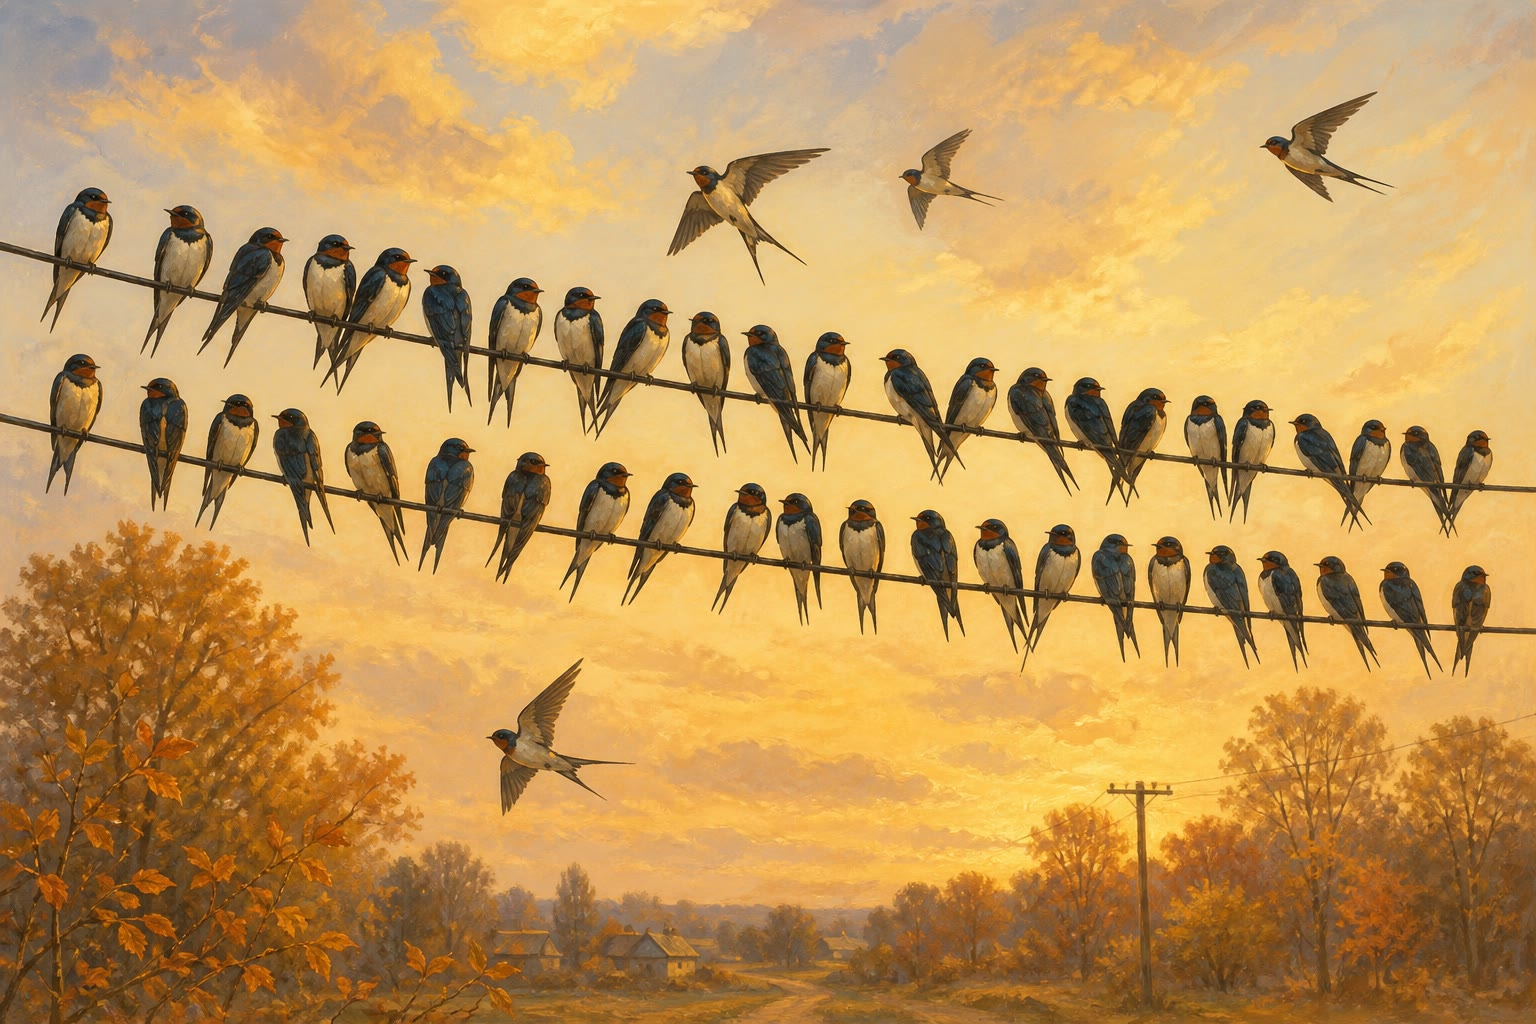
\includegraphics[width=0.62\linewidth]{images/book1/ai/g3-seasons-swallows.jpg}

{\small Octobre sur les fils~: les hirondelles se rassemblent pour
le départ, quelques jours avant que les \omterm{prop:g3:sorting-living-things:groups}{insectes} ne manquent.}
\end{omfigure}

\section{Trois réponses à l'hiver}

\begin{definition}[Migration]\label{def:g3:animals-through-seasons:migration}
\emph{Migrer}\index{migrer}, c'est voyager chaque année d'une région
à une autre au fil des saisons --- partir avant l'hiver vers des
terres plus chaudes où la nourriture demeure, et revenir au
printemps. L'hirondelle, la cigogne et la grue sont des
\emph{migrateurs}\index{migration}~; certains parcourent des
milliers de kilomètres, et retrouvent leur chemin jusqu'au même nid.
\end{definition}

\begin{definition}[Hibernation]\label{def:g3:animals-through-seasons:hibernation}
\emph{Hiberner}\index{hiberner}, c'est passer l'hiver dans un
\omterm{prop:g1:healthy-habits:needs}{sommeil} profond et froid, caché dans un abri~: le corps se
refroidit, le cœur et la respiration ralentissent jusqu'à presque
rien, et l'\omterm{def:g1:animals-around-us:animal}{animal} vit lentement sur la graisse accumulée en automne.
Le hérisson, le loir, la marmotte et la chauve-souris hibernent.
\end{definition}

\begin{definition}[Rester actif]\label{def:g3:animals-through-seasons:active}
Les autres \emph{restent actifs}\index{rester actif (en hiver)} et
changent d'équipement ou d'habitudes~: un \emph{pelage
d'hiver}\index{pelage d'hiver} plus épais, des
\emph{réserves}\index{réserve de nourriture} amassées en automne
(les noisettes enterrées de l'écureuil), un changement de menu (le
merle de \cref{ex:g2:what-animals-eat:winter}), ou simplement des
recherches plus acharnées --- le renard, le chevreuil, le
rouge-gorge.
\end{definition}

\begin{omfigure}
\begin{tikzpicture}
  \draw[thick, omDef, fill=omDef!7, rounded corners=6pt]
    (0,0) rectangle (4.1,3.1);
  \draw[thick, omProp, fill=omProp!7, rounded corners=6pt]
    (4.5,0) rectangle (8.6,3.1);
  \draw[thick, omMeth, fill=omMeth!7, rounded corners=6pt]
    (9.0,0) rectangle (13.1,3.1);
  \node[font=\small\bfseries, omDef, text height=1.6ex, text depth=0.4ex]
    at (2.05,2.75) {migrer};
  \node[font=\small\bfseries, omProp, text height=1.6ex, text depth=0.4ex]
    at (6.55,2.75) {hiberner};
  \node[font=\small\bfseries, omMeth, text height=1.6ex, text depth=0.4ex]
    at (11.05,2.75) {rester actif};
  \node[font=\small, align=center, text width=3.8cm] at (2.05,1.2)
    {partir vers des terres\\ où la nourriture reste\\[2pt] hirondelle, cigogne,\\ grue};
  \node[font=\small, align=center, text width=3.8cm] at (6.55,1.2)
    {sommeil froid profond,\\ sur la graisse accumulée\\[2pt] hérisson, marmotte,\\ loir, chauve-souris};
  \node[font=\small, align=center, text width=3.8cm] at (11.05,1.2)
    {pelage d'hiver, réserves,\\ nouveau menu, recherche\\[2pt] renard, écureuil,\\ rouge-gorge, chevreuil};
\end{tikzpicture}

{\small Trois façons de traverser le même hiver. Chacune résout
autrement le double problème --- la chaleur et la nourriture.}
\end{omfigure}

\begin{example}[Trois voisins, trois stratégies]\label{ex:g3:animals-through-seasons:three}
Une haie en janvier~: les hirondelles qui nichaient au-dessus sont
en Afrique, à attraper des \omterm{prop:g3:sorting-living-things:groups}{insectes} sous un soleil chaud~; le
hérisson d'en bas dort, froid et ralenti, dans son nid de \omterm{def:g1:plants-around-us:parts}{feuilles},
en brûlant la graisse d'août~; le rouge-gorge du dessus, dans son
plumage d'hiver ébouriffé, patrouille à la recherche des dernières
baies. En avril, tous les trois s'affaireront de nouveau dans la
même haie.
\end{example}

\begin{remark}[Dormir n'est pas paresser, voyager n'est pas du tourisme]\label{rem:g3:animals-through-seasons:cost}
Chaque stratégie a son prix. Le migrateur risque un voyage
épuisant~; l'hibernant doit amasser chaque gramme de sa graisse
d'hiver en automne --- un hérisson trop maigre en novembre ne se
réveillera pas au printemps~; l'\omterm{def:g1:animals-around-us:animal}{animal} actif parie sur le fait de
trouver à manger pendant les mois les plus affamés. L'hiver se paie
d'avance, ou en route, ou jour après jour.
\end{remark}

\begin{method}[Deviner la stratégie d'hiver d'un animal]\label{met:g3:animals-through-seasons:guess}
\begin{enumerate}
  \item Demande-toi ce qu'il mange, et si cette nourriture existe
        ici en hiver~;
  \item nourriture complètement disparue (\omterm{prop:g3:sorting-living-things:groups}{insectes} volants,
        nectar)~: attends-toi à une \omterm{def:g3:animals-through-seasons:migration}{migration} ou à une
        hibernation~;
  \item nourriture trouvable (\omterm{prop:g3:flowers-fruits-seeds:transform}{graines}, baies, proies)~: attends-toi
        à un hiver actif, peut-être avec un \omterm{def:g1:animals-around-us:covering}{pelage} plus épais ou
        des réserves~;
  \item vérifie en automne~: s'engraisser et creuser un nid annonce
        l'hibernation~; se rassembler en groupes annonce le départ.
\end{enumerate}
\end{method}

\begin{example}[Le printemps défait tout]\label{ex:g3:animals-through-seasons:spring}
En mars et en avril, l'ordre s'inverse~: les \omterm{prop:g3:sorting-living-things:groups}{insectes} reviennent,
les \omterm{def:g3:animals-through-seasons:migration}{migrateurs} reparaissent à leurs anciens nids, les hibernants se
réveillent maigres et affamés, les \omterm{def:g3:animals-through-seasons:active}{pelages d'hiver} tombent. Les
saisons tournent, et le calendrier des \omterm{def:g1:animals-around-us:animal}{animaux} tourne avec elles ---
l'automne prochain, les hirondelles s'aligneront de nouveau sur les
fils.
\end{example}

\section{Exercices}

\begin{exercise}[$\star$]\label{exo:g3:animals-through-seasons:1}
Quel double problème l'hiver pose-t-il à chaque \omterm{def:g1:animals-around-us:animal}{animal}~?
\end{exercise}

\begin{exercise}[$\star$]\label{exo:g3:animals-through-seasons:2}
Nomme les trois stratégies d'hiver, avec deux \omterm{def:g1:animals-around-us:animal}{animaux} pour chacune.
\end{exercise}

\begin{exercise}[$\star$]\label{exo:g3:animals-through-seasons:3}
Qu'arrive-t-il au corps d'un hérisson qui hiberne pendant son long
\omterm{prop:g1:healthy-habits:needs}{sommeil}~? De quoi vit-il~?
\end{exercise}

\begin{exercise}[$\star$]\label{exo:g3:animals-through-seasons:4}
Pourquoi l'hirondelle doit-elle partir, exactement --- quelle est sa
nourriture, et que devient-elle ici en hiver~?
\end{exercise}

\begin{exercise}[$\star$]\label{exo:g3:animals-through-seasons:5}
Donne trois façons dont un \omterm{def:g1:animals-around-us:animal}{animal} actif traverse l'hiver, chacune
avec son \omterm{def:g1:animals-around-us:animal}{animal}.
\end{exercise}

\begin{exercise}[$\star$]\label{exo:g3:animals-through-seasons:6}
Quel est le prix de chaque stratégie, d'après
\cref{rem:g3:animals-through-seasons:cost}~?
\end{exercise}

\begin{exercise}[$\star$]\label{exo:g3:animals-through-seasons:7}
En automne, on voit un \omterm{def:g1:animals-around-us:animal}{animal} manger énormément et garnir un trou de
\omterm{def:g1:plants-around-us:parts}{feuilles} sèches. Quelle stratégie prépare-t-il~? Quelle étape de
\cref{met:g3:animals-through-seasons:guess} te l'a dit~?
\end{exercise}

\begin{exercise}[$\star$]\label{exo:g3:animals-through-seasons:8}
À toi d'essayer~: tiens une liste d'hiver des \omterm{prop:g3:sorting-living-things:groups}{oiseaux} que tu vois
vraiment dehors pendant une semaine froide. Les hirondelles y
sont-elles~? Lesquels de tes \omterm{prop:g3:sorting-living-things:groups}{oiseaux} ont choisi la stratégie active~?
\end{exercise}

\begin{exercise}[$\star\star$]\label{exo:g3:animals-through-seasons:9}
Applique \cref{met:g3:animals-through-seasons:guess} à~: (a)
l'écureuil (il mange noisettes et \omterm{prop:g3:flowers-fruits-seeds:transform}{graines})~; (b) la grue (elle mange
grenouilles et \omterm{prop:g3:sorting-living-things:groups}{insectes} des prés humides). Que fait probablement
chacun en hiver~?
\end{exercise}

\begin{exercise}[$\star\star$]\label{exo:g3:animals-through-seasons:10}
Un automne doux garde un jeune hérisson éveillé et en chasse
tardive, mais il reste maigre. Pourquoi est-ce dangereux pour lui,
d'après \cref{rem:g3:animals-through-seasons:cost}~? Que font les
centres de soins avec les hérissons trop maigres en automne~?
\end{exercise}
